\paragraph{Sawing}

\begin{figure}[ht]
    \centering
    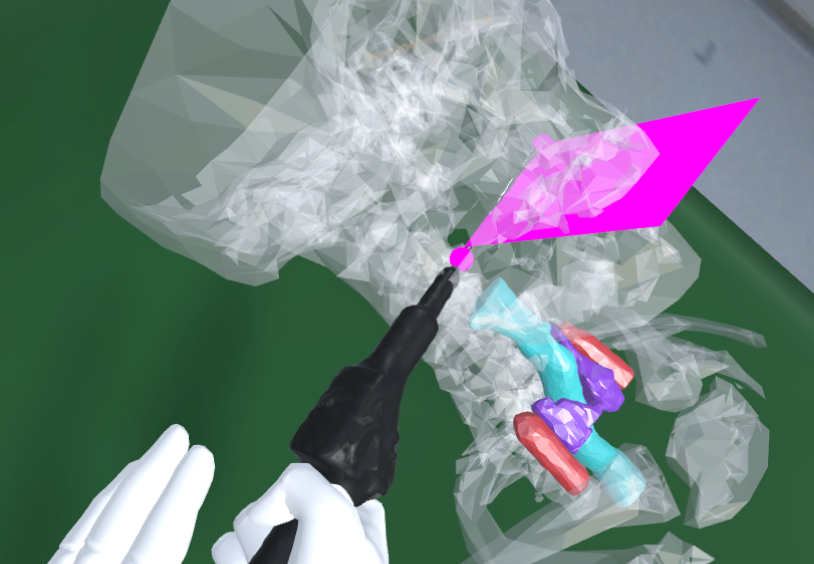
\includegraphics[width=200px]{images/implementation/features/procedures/bonesaw.png}
    \caption{\label{fig::FeatureBoneSaw}Bonesaw procedure. Left: The procedure is started by pressing down the "perform" button. Indications show two starting points which are 
    used to create the plane when letting go of the button. Right: The button has been released and as plane visualizing the procedure has been created.}
\end{figure}

The \textbf{sawing} procedure is performed by picking up the bonesaw.
The indications to the user consist of two spheres indicating the start and end of the cutting plane (Figure \ref{fig::FeatureBoneSaw}).
These indicators are placed at the top and bottom end of the cutting portion of the bonesaws blade.
The procedure is triggered by first pressing down the "perform" button and holding it.
When letting go of the button, a two dimensional plane is created in the three dimensional space by using four points.
Two of these points are stored internally when pressing down, and the other two when letting go of the trigger button.
A plane is then created and added to the project case.

\begin{figure}[ht]
    \centering
    
\includegraphics[width=200px]{images/todo.png}
    \caption{\label{fig::MultipleSawing}Cutting of the lower jaw simulated by performing two sawing procedures in succession.}
\end{figure}

Through following the plane with the bonesaw, the user can reproduce the way in which the bonesaw has been moved.
More complex cutting procedures can be simulated by breaking them down into two-dimensional shapes and performing multiple operational steps, as depicted in Figure \ref{fig::MultipleSawing}.